\chapter{Coupling Discrete Dislocation Dynamics to Finite Element Methods}
\label{c:ddd_fem}
\section{Superposition Scheme}
\label{s:sup_sch}
Coupling discrete dislocation dynamics to a finite element method \cite{analytic_tractions} is important to properly simulate micromechanical tests because discrete dislocation dynamics provides us with a more precise set of inputs and greater granularity for solving the finite element problem. This can be achieved by using a so-called superposition scheme \cref{f:fem_ddd} that enables the independent solution of both problems, whilst feeding information from one to the other in a continuous feedback loop.
\begin{figure}
	\centering
	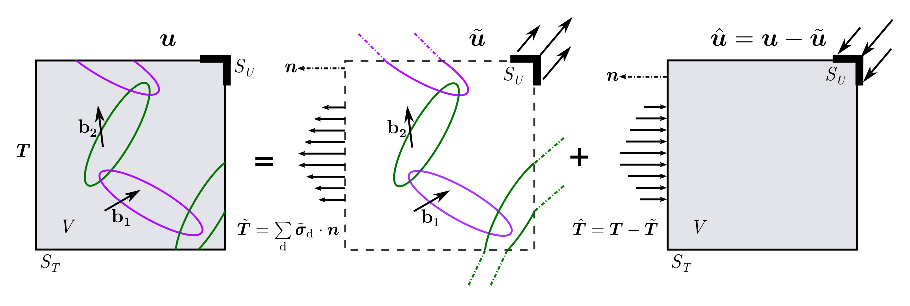
\includegraphics[width=\linewidth]{fem_ddd.eps}
	\caption[Coupling Discrete Dislocation Dynamics to Finite Element Methods.]{The dislocation ensemble in a volume $ V $ is bounded by surface $ S $. First, the traction field $ \sum_{\textrm{d}} \tns{\tilde{\sigma}}_{\textrm{d}} $ due to the dislocation ensemble is evaluated at the surface. Then, a traditional finite element method or boundary element method calculates the image traction field $ \tns{\hat{\sigma}} \times \vec{n} $. Which is then fed back to the discrete dislocation dynamics problem to evolve the dislocation positions and repeat the cycle. Image edited from \cite{analytic_tractions}.}
	\label{f:fem_ddd}
\end{figure}
\section{Extracting Surface Nodes}
The finite element method coupler arranges the nodes starting on the $ xz $-plane where $ y \in \{0 \to n~\mathrm{d}y\}$ and $n\in \mathbb{N} $. However in order to couple discrete dislocation dynamics to finite element method we only require the surface nodes where displacements are not calculated. Because we're working with rectangular prisms, we can easily pick out the surface nodes using a search algorithm with a logical mask. MATLAB and Fortran provide vector intrinsics that allow one to do so. \Cref{f:fem_surf_nodes} illustrates only the surface nodes according to our implementation's node arrangement---which is the $ xz $-plane whose domain is $[y_{\text{min}},~ y_{\text{max}}]$.
\begin{figure}
	\centering
	\begin{subfigure}[b]{0.45\linewidth}
		\centering
		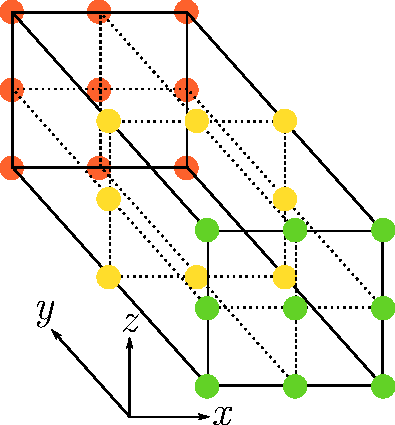
\includegraphics[width=\linewidth]{fem_surf_nodes.pdf}
		\caption[Surface nodes of our finite element model.]{Arrangement of the surface nodes of our finite element model. finite element nodes are arranged in chunks of $ \Delta x \Delta z $ nodes in our implementation, but we only want the surface nodes.}
		\label{f:fem_surf_nodes}
	\end{subfigure}
	~
	\begin{subfigure}[b]{0.45\linewidth}
		\centering
		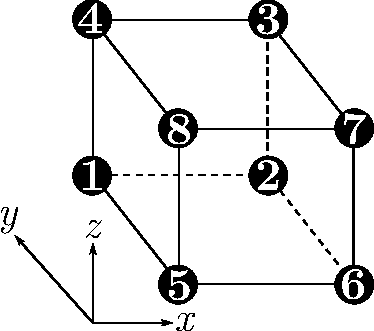
\includegraphics[width=\linewidth]{fe_numbering.pdf}
		\caption[Single finite element node numbering.]{Single finite element node numbering. It is necessary to know which finite element plane corresponds to which node labels. This lets us design the auxiliary matrix that selects nodes according to the planes we want to extract.}
		\label{f:fe_numbering}
	\end{subfigure}
	\caption[Finite Element node arrangement for coupling to Discrete Dislocation Dynamics.]{finite element node arrangement for coupling to discrete dislocation dynamics.}
	\label{f:fem_node_arr}
\end{figure}
However, due to the nature of the analytical solutions in \cref{c:lin_rect}, we need all the surface nodes of the rectangular faces for which there are no displacements. This means that edge nodes are shared between 2 adjacent faces and corner nodes between 3 adjacent faces. In order to properly apply the logical mask to find \emph{only} the surface nodes need to know that each finite element's nodes are numbered according to \cref{f:fe_numbering}.

Using \cref{f:fem_node_arr} one can work out which nodes are of interest to whichever surface is being extracted. The ordering of the nodes in the final array will depend on the definition of the problems in \cref{c:lin_rect}.

Node selection remains an expensive operation and minimising array indexing is of the utmost importance for the best perfomance. Selecting nodes in the traditional sense, i.e. with code branching such as \texttt{if statements} or \texttt{case selection} is unmantainable, verbose and very prone to mistakes. The issue was solved by introducing an auxiliary matrix which defines various parameters that aid node selection and greatly reduces code size, improves readability, and eliminates the need for code branching. The matrix can be constructed utilising \cref{f:fem_node_arr} in order to know which nodes correspond to which finite element planes. The $ p\textsuperscript{th} $ column of the matrix\footnote{MATLAB uses column-major ordering, so this gives us the best performance for vectorised code.} corresponds to the $ p\textsuperscript{th} $ plane (according to an arbitrary plane numbering) and is defined as,
\begin{align}\label{eq:surf_node_util_vec}
	\vec{V_{p}}^{\mathsf{T}} =
	\begin{bmatrix}
		L_{1p} & L_{2p} & \cdots & L_{Np} & A_{p} & C_{p}
	\end{bmatrix}\,,
\end{align}
where $ L_{np} $ is the numeric label for node $ n $ as given by \cref{f:fem_node_arr}, $ A_{p} $ is the area of the plane, and $ C_{p} $ is the numeric label of the orthogonal coordinate to the plane $ C_{p} = 1, ~2, ~3 $ for the $ x, ~y, ~z $ coordinates respectively. $ A_{p} $ lets us segment our output and transitional arrays so that the only data being modified is that which corresponds to the correct plane and $ C_{p} $ lets us know which coordinate we must use in our selection criteria. Using our particular node labelling scheme (with dimensions $ \Delta x,~ \Delta y,~ \Delta z $ respectively in the $ x,~ y,~ z $ directions), the matrix is defined as,
\begin{align}\label{eq:surf_node_util}
	\mtx{V} =
	\begin{bmatrix}
		5                 & 2                 & 6                 & 1                 & 5                 & 4                 \\
		1                 & 6                 & 5                 & 2                 & 6                 & 3                 \\
		8                 & 3                 & 7                 & 4                 & 1                 & 8                 \\
		4                 & 7                 & 8                 & 3                 & 2                 & 7                 \\
		\Delta y \Delta z & \Delta y \Delta z & \Delta x \Delta z & \Delta x \Delta z & \Delta x \Delta y & \Delta x \Delta y \\
		1                 & 1                 & 2                 & 2                 & 3                 & 3
	\end{bmatrix}\,.
\end{align}
The information codified in \cref{eq:surf_node_util} lets us index and process only the necessary columns to extract the surface nodes we're interested in. The advantage of this setup over a naïve implementation is that it can be relatively easily expanded, maintained, and is general enough that it lends itself to a variety of selection criteria. The columns from left to right (1 to 6) represent:
\begin{inparaenum}[{face} 1 $ \equiv $]
	\item $ \min(x),~ yz $-plane;
	\item $ \max(x),~ yz $-plane;
	\item $ \min(y),~ xz $-plane;
	\item $ \max(y),~ xz $-plane;
	\item $ \min(z),~ xy $-plane;
	\item $ \max(z),~ xy $-plane.
\end{inparaenum}

It is important to make sure the nodes are extracted in a self consistent manner because the problem definitions in \cref{c:lin_rect} assume a specific node ordering. In particular, the labelling chirality must remain the same. This is due to the fact that the problems in \cref{c:lin_rect} utilise internal coordinates derived from a set of basis vectors, and scalar projections onto them. If the relationship between the vectors is kept, but the chirality is different (opposite) the calculated quantities will have the wrong sign. If however the relationship between the vectors is different to the problem formulation, the program will crash due to division by 0. Self-consistency was achieved by placing an imaginary observer inside the finite element model facing the $ \min(x),~ yz $-plane (face 1) and rotating it to view all 6 planes according to \cref{f:surf_node_plane}.
\begin{figure}
	\centering
	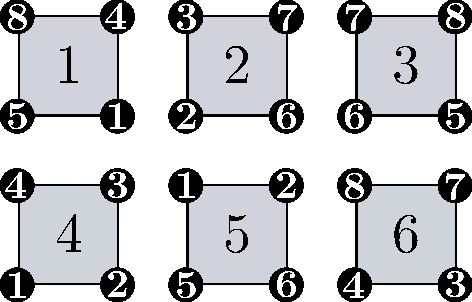
\includegraphics[width=0.75\linewidth]{surf_node_plane.pdf}
	\caption[Self-consistent, chirality preserving surface planes.]{Self-consistent, chirality preserving surface planes. Plane and node numbering according to the columns of \cref{eq:surf_node_util} and \cref{f:fem_node_arr}.}
	\label{f:surf_node_plane}
\end{figure}
\section{Mapping Forces}
\begin{algorithm}
	\caption{If $ \vec{\hat{F}} $'s columns are arranged the same way as $ \vec{\gamma_{t}} $.}
	\begin{algorithmic}[1]
		\State\Comment{Loop through the array containing the node labels of the relevant surface nodes.}
		\For{$ i = 0;\, i < \rvar{length}(\vec{\gamma_{t}});\, i++$}
		\State\Comment{Save the global node label for the current iteration.}
		\State $ n \gets \vec{\gamma_{t}}[i] $
		\State\Comment{Use the node label to find a vector with the linearised index of all surface nodes whose labels correspond to the node whose forces we want to pass on to the finite element method coupler.}
		\State $ \vec{L} \gets \rvar{find}(\mtx{N_{L}} == n) $
		\State\Comment{Loop over coordinates.}
		\For{$ k = 0;\, k < 3;\, k++ $}
		\State\Comment{Use global node label vector to index the force array from the analytical force calculation due to dislocations on surface nodes. Multiplied by 3 because there are three coordinates per node. We sum the forces from the analytical calculation because the same global node can be part of multiple surface elements. We add $ k $ because the $ x,~y,~z $ coordinates are consecutively stored in $ \mtx{F_{n}} $.}
		\State $ \mtx{\hat{F}}[3\times \vec{L} + k] \gets \mtx{\hat{F}}[3\times \vec{L} + k] + \sum\mtx{F_{n}}[3\times \vec{L} + k]  $
		\EndFor
		\EndFor
	\end{algorithmic}
\end{algorithm}

%	\begin{algorithm}
%		\begin{algorithmic}[1]
%			content...
%		\end{algorithmic}
%	\end{algorithm}
\begin{figure}
	\centering
	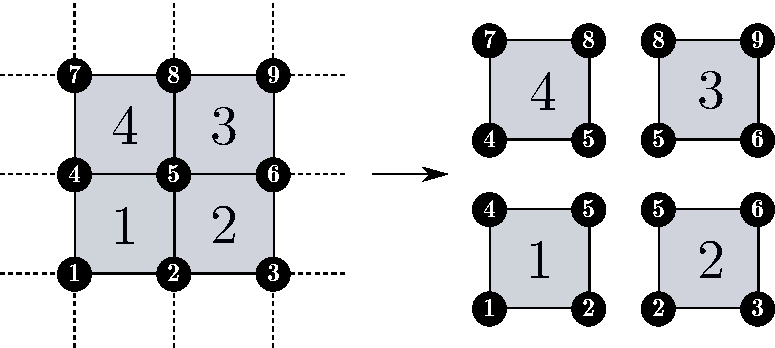
\includegraphics[width=\linewidth]{lrse_thread_map.pdf}
	\caption[Finite element nodes shared by multiple surface elements.]{finite element nodes shared by multiple surface elements.}
	\label{f:fe_node_share}
\end{figure}

$ \vec{\hat{F}} $ only cares about the global node numbers, of which there are $ M $. The columns of $ \mtx{N_{L}},~ \mtx{F_{N}} $ represent the 4 nodes of a surface element, the rows represent the surface element they are part of. The column vector $ \vec{x} $ represents the $ x,~y,~z$-coordinates of the node-element or global node corresponding to their subscript. The column vector $ \vec{\gamma_{t}} $ is the list of global nodes for which the forces induced by dislocations must be calculated.
\begin{align}
	\vec{x_{e,n}}^{\mathsf{T}} & \equiv	\begin{bmatrix}
		x_{en} & y_{en} & z_{en}
	\end{bmatrix}, \quad
	\vec{\hat{x}_{n}}^{\mathsf{T}} \equiv	\begin{bmatrix}
		x_{n} & y_{n} & z_{n}
	\end{bmatrix}      \\
	\begin{split}
		\mtx{N_{L}} &=	\begin{bmatrix}
			l_{1,1} & l_{1,2} & l_{1,4} & l_{1,5} \\
			l_{2,2} & l_{2,3} & l_{2,5} & l_{2,6} \\
			l_{3,5} & l_{3,6} & l_{3,8} & l_{3,9} \\
			l_{4,4} & l_{4,5} & l_{4,7} & l_{4,8} \\
		\end{bmatrix}
	\end{split}
	, \quad
	\vec{\gamma} =   \begin{bmatrix}
		l_1    \\
		l_2    \\
		\vdots \\
		l_9
	\end{bmatrix}                          \\
	\begin{split}
		\mtx{F_{e}} &=	\begin{bmatrix}
			\vec{x_{1,1}} & \vec{x_{1,2}} & \vec{x_{1,3}} & \vec{x_{1,4}} \\
			\vec{x_{2,1}} & \vec{x_{2,2}} & \vec{x_{2,3}} & \vec{x_{2,4}} \\
			\vec{x_{3,1}} & \vec{x_{3,2}} & \vec{x_{3,3}} & \vec{x_{3,4}} \\
			\vec{x_{4,1}} & \vec{x_{4,2}} & \vec{x_{4,3}} & \vec{x_{4,4}} \\
		\end{bmatrix}
	\end{split}
	,\quad
	\vec{\hat{F}} = 	\begin{bmatrix}
		\vec{\hat{x}_{1}} \\
		\vec{\hat{x}_{2}} \\
		\vec{\hat{x}_{3}} \\
		\vec{\hat{x}_{4}}
	\end{bmatrix}\,.\label{eq:force_imp}
\end{align}

